\subsection{Damping Implementation}\label{damping implementation}
    ``Damped distribution functions'' are incorporated in this work into {\tt GENE} similarly how one would any other distribution function: with a new {\tt dist\_eq\_*\_damped\_t} class (in a {\tt dist\_eq\_*\_damped\_m} module) extending {\tt dist\_eq\_t}. Whereas a traditional background distribution needs only its distribution function, $f_{s0}$ (or more accurately its distribution function's parameters, $n_{s}$, $u_{\parallel s}$, $T_{s}$, etc.) to be defined, a damped distribution requires (as highlighted in subsection \ref{damped distributions}) 3 ``ingredients'':
    \begin{itemize}
        \item  $f_{s0}^{\rm pre}\left[\psi; v_{\parallel}^{\rm pre}, \mu^{\rm pre}\right]$ (or more accurately the parameters, $n_{s}$, $u_{\parallel s}$, $T_{s}$, etc. of) the velocity distribution \emph{before damping}.
        \item  $v_{\parallel}^{\rm pre}(v_{\parallel}, \mu)$, the parallel velocity a damped particle had \emph{before damping}.
        \item  $\mu^{\rm pre}(v_{\parallel}, \mu)$, the magnetic moment a damped particle had \emph{before damping}.
    \end{itemize}
    Within the implementation, therefore, a class/module for a \emph{damped} distribution looks almost identical to one for a \emph{non-damped} distribution, except for its definition containing a new variable that carries information on the damping function, $(v_{\parallel}, \mu)  \mapsto  (v_{\parallel}^{\rm pre}, \mu^{\rm pre})$. This is done through:
    \begin{enumerate}
        \item  General implementation of the new class, {\tt damping\_t} (in the {\tt damping\_base\_m} module), the class of damping functions, with space all the relevant information on the damping function.
        \item  User implementation of a new class, {\tt damping\_*\_t} (in a {\tt damping\_*\_m} module), extending {\tt damping\_t}, for each specific damping function—say, \emph{uniform} damping, as defined in subsection \ref{damped distributions}—the user would like to consider, defining the damping function $(v_{\parallel}, \mu)  \mapsto  (v_{\parallel}^{\rm pre}, \mu^{\rm pre})$ in consideration.
        \item  User implementation of a new subclass {\tt dist\_eq\_*\_damped\_t} (in a {\tt dist\_eq\_*\_damped\_m} module), extending {\tt dist\_eq\_t}, just as one might do already to implement a new distribution, except this time containing (and initializing) a new variable {\tt dist\_eq\_*\_damped\%damp} of type {\tt damping\_*\_t} containing information on the damping function in question.
    \end{enumerate}
    This new class structure is highlighted in {\color{red!90} red} in Figure \ref{class structure after damping}.
    
    \begin{figure}[!h]
    \centering
    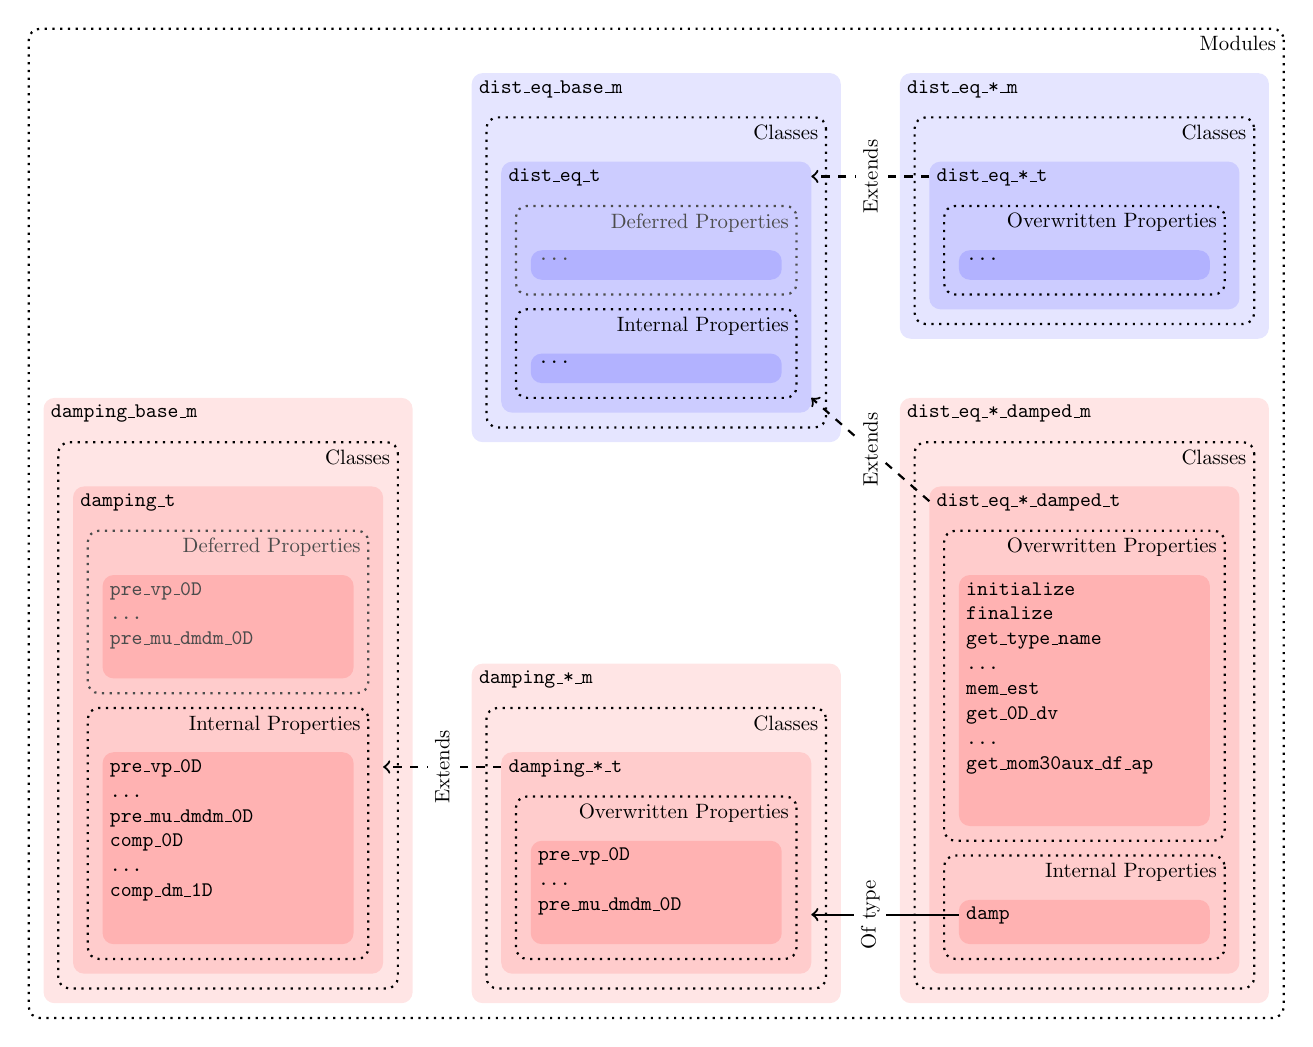
\begin{tikzpicture}[scale = 0.75, every node/.style = {scale = 0.75}, every text node part/.style = {align = left}]
        \draw[rounded corners, dotted, thick]
            (13.75, 0.75) node[below left] {Modules}
            rectangle
            (-7.5, -16);
            \fill[rounded corners, fill = blue!10]
                (0, 0) node[below right] {\tt dist\_eq\_base\_m}
                rectangle
                (6.25, -6.25);
                \draw[rounded corners, dotted, thick]
                    (6, -0.75) node[below left] {Classes}
                    rectangle
                    (0.25, -6);
                    \fill[rounded corners, fill = blue!20]
                        (0.5, -1.5) node[below right] {\tt dist\_eq\_t}
                        rectangle
                        (5.75, -5.75);
                        \draw[rounded corners, dotted, thick, dotted, black!70]
                            (5.5, -2.25) node[below left] {Deferred Properties}
                            rectangle
                            (0.75, -3.75);
                            \fill[rounded corners, fill = blue!30]
                                (1, -3) node[below right] {}
                                rectangle
                                (5.25, -3.5);
                            \node[black!70] at (1, -3) [below right] {
                                    {\tt ...}
                                };
                        \draw[rounded corners, dotted, thick]
                            (5.5, -4) node[below left] {Internal Properties}
                            rectangle
                            (0.75, -5.5);
                            \fill[rounded corners, fill = blue!30]
                                (1, -4.75) node[below right] {}
                                rectangle
                                (5.25, -5.25);
                            \node at (1, -4.75) [below right] {
                                    {\tt ...}
                                };
            \fill[rounded corners, fill = blue!10]
                (7.25, 0) node[below right] {\tt dist\_eq\_*\_m}
                rectangle
                (13.5, -4.5);
                \draw[rounded corners, dotted, thick]
                    (13.25, -0.75) node[below left] {Classes}
                    rectangle
                    (7.5, -4.25);
                    \fill[rounded corners, fill = blue!20]
                        (7.75, -1.5) node[below right] {\tt dist\_eq\_*\_t}
                        rectangle
                        (13, -4);
                        \draw[rounded corners, dotted, thick]
                            (12.75, -2.25) node[below left] {Overwritten Properties}
                            rectangle
                            (8, -3.75);
                            \fill[rounded corners, fill = blue!30]
                                (8.25, -3) node[below right] {}
                                rectangle
                                (12.5, -3.5);
                            \node at (8.25, -3) [below right] {
                                    {\tt ...}
                                };
            \fill[rounded corners, fill = red!10]
                (-7.25, -5.5) node[below right] {\tt damping\_base\_m}
                rectangle
                (-1, -15.75);
                \draw[rounded corners, dotted, thick]
                    (-1.25, -6.25) node[below left] {Classes}
                    rectangle
                    (-7, -15.5);
                    \fill[rounded corners, fill = red!20]
                        (-6.75, -7) node[below right] {\tt damping\_t}
                        rectangle
                        (-1.5, -15.25);
                        \draw[rounded corners, dotted, thick, dotted, black!70]
                            (-1.75, -7.75) node[below left] {Deferred Properties}
                            rectangle
                            (-6.5, -10.5);
                            \fill[rounded corners, fill = red!30]
                                (-6.25, -8.5) node[below right] {}
                                rectangle
                                (-2, -10.25);
                            \node[black!70] at (-6.25, -8.5) [below right] {
                                    {\tt pre\_vp\_0D} \\
                                    {\tt ...} \\
                                    {\tt pre\_mu\_dmdm\_0D}
                                };
                        \draw[rounded corners, dotted, thick]
                            (-1.75, -10.75) node[below left] {Internal Properties}
                            rectangle
                            (-6.5, -15);
                            \fill[rounded corners, fill = red!30]
                                (-6.25, -11.5) node[below right] {}
                                rectangle
                                (-2, -14.75);
                            \node at (-6.25, -11.5) [below right] {
                                    {\tt pre\_vp\_0D} \\
                                    {\tt ...} \\
                                    {\tt pre\_mu\_dmdm\_0D}  \\
                                    {\tt comp\_0D} \\
                                    {\tt ...} \\
                                    {\tt comp\_dm\_1D}
                                };
            \fill[rounded corners, fill = red!10]
                (0, -10) node[below right] {\tt damping\_*\_m}
                rectangle
                (6.25, -15.75);
                \draw[rounded corners, dotted, thick]
                    (6, -10.75) node[below left] {Classes}
                    rectangle
                    (0.25, -15.5);
                    \fill[rounded corners, fill = red!20]
                        (0.5, -11.5) node[below right] {\tt damping\_*\_t}
                        rectangle
                        (5.75, -15.25);
                        \draw[rounded corners, dotted, thick]
                            (5.5, -12.25) node[below left] {Overwritten Properties}
                            rectangle
                            (0.75, -15);
                            \fill[rounded corners, fill = red!30]
                                (1, -13) node[below right] {}
                                rectangle
                                (5.25, -14.75);
                            \node at (1, -13) [below right] {
                                    {\tt pre\_vp\_0D} \\
                                    {\tt ...} \\
                                    {\tt pre\_mu\_dmdm\_0D}
                                };
            \fill[rounded corners, fill = red!10]
                (7.25, -5.5) node[below right] {\tt dist\_eq\_*\_damped\_m}
                rectangle
                (13.5, -15.75);
                \draw[rounded corners, dotted, thick]
                    (13.25, -6.25) node[below left] {Classes}
                    rectangle
                    (7.5, -15.5);
                    \fill[rounded corners, fill = red!20]
                        (7.75, -7) node[below right] {\tt dist\_eq\_*\_damped\_t}
                        rectangle
                        (13, -15.25);
                        \draw[rounded corners, dotted, thick]
                            (12.75, -7.75) node[below left] {Overwritten Properties}
                            rectangle
                            (8, -13);
                            \fill[rounded corners, fill = red!30]
                                (8.25, -8.5) node[below right] {}
                                rectangle
                                (12.5, -12.75);
                            \node at (8.25, -8.5) [below right] {
                                    {\tt initialize} \\
                                    {\tt finalize} \\
                                    {\tt get\_type\_name} \\
                                    {\tt ...} \\
                                    {\tt mem\_est} \\
                                    {\tt get\_0D\_dv} \\
                                    {\tt ...} \\
                                    {\tt get\_mom30aux\_df\_ap}
                                };
                        \draw[rounded corners, dotted, thick]
                            (12.75, -13.25) node[below left] {Internal Properties}
                            rectangle
                            (8, -15);
                            \fill[rounded corners, fill = red!30]
                                (8.25, -14) node[below right] {}
                                rectangle
                                (12.5, -14.75);
                            \node at (8.25, -14) [below right] {
                                    {\tt damp}
                                };
        \draw[->, thick, dashed]
            (7.75, -1.75) -- (5.75, -1.75)
            node[midway, rotate = 90, fill = white] {Extends};
        \draw[->, thick, dashed]
            (7.75, -7.25) -- (5.75, -5.5)
            node[midway, rotate = 90, fill = white] {Extends};
        \draw[->, thick, dashed]
            (0.5, -11.75) -- (-1.5, -11.75)
            node[midway, rotate = 90, fill = white] {Extends};
        \draw[->, thick]
            (8.25, -14.25) -- (5.75, -14.25);
            \node[rotate = 90, fill = white] at (6.75, -14.25) {Of type};
    \end{tikzpicture}
    \caption{{\tt GENE} equilibrium distribution class structure \emph{after} addition of damping modules. Base modules marked in {\color{blue!90} blue}, additions marked in {\color{red!90} red}.}
    \label{class structure after damping}
\end{figure}

    As for what information should be contained in the {\tt damping\_t} class, consider what information is needed about the damping function to evaluate all the procedures in Figure \ref{distribution procedures}. Since both {\tt get\_*D\_dvdm} and the terms in the last two sections can be written\footnote{if they cannot be evaluated directly} in terms of those in the first section, and the only component of {\tt get\_edr} that changes between distribution function classes is that which is featured in {\tt get\_edr\_prefactor}, the only 3 terms that actually need evaluating to implement a new distribution function class are simply the 3 derivatives of $f_{s0}$ in $v_{\parallel}$, $\mu$, $\psi$:
    \begin{center}\begin{tabular}{ c | c }
        Procedure  &  Functional  \\
        \hline\hline
        {\tt get\_*D\_dv}  &  $\partial_{v_{\parallel}}f_{s0}$  \\
        \hline
        {\tt get\_*D\_dm}  &  $\partial_{\mu}f_{s0}$  \\
        \hline\hline
        {\tt get\_edr\_prefactor}  &  $\partial_{\psi}f_{s0}$ (without $B$ derivative?)
    \end{tabular}\end{center}
    Recall then equation (\ref{damped distribution function}) for $f_{s0}$
    \begin{equation*}
        f_{s0}[\psi; v_{\parallel}, \mu]  =  J(v_{\parallel}, \mu)f_{s0}^{\rm pre}\left[\psi; v_{\parallel}^{\rm pre}(v_{\parallel}, \mu), \mu^{\rm pre}(v_{\parallel}, \mu)\right]
    \end{equation*}
    alongside equation (\ref{Jacobian}) for $J$
    \begin{equation*}
        J(v_{\parallel}, \mu)  :=  \partial_{v_{\parallel}}v_{\parallel}^{\rm pre}(v_{\parallel}, \mu)\partial_{\mu}\mu^{\rm pre}(v_{\parallel}, \mu) - \partial_{\mu}v_{\parallel}^{\rm pre}(v_{\parallel}, \mu)\partial_{v_{\parallel}}\mu^{\rm pre}(v_{\parallel}, \mu)
    \end{equation*}
    The 3 relevant derivatives in $f_{s0}$ then evaluate as:
    \begin{align}
        \partial_{v_{\parallel}}f_{s0}
            &=  \partial_{v_{\parallel}}J\cdot f_{s0}^{\rm pre}
            + J\cdot\left(\partial_{v_{\parallel}^{\rm pre}}f_{s0}^{\rm pre}\cdot\partial_{v_{\parallel}}v_{\parallel}^{\rm pre}
            + \partial_{\mu^{\rm pre}}f_{s0}^{\rm pre}\cdot\partial_{v_{\parallel}}\mu^{\rm pre}\right)  \\
        \partial_{\mu}f_{s0}
            &=  \partial_{\mu}J\cdot f_{s0}^{\rm pre}
            + J\cdot\left(\partial_{v_{\parallel}^{\rm pre}}f_{s0}^{\rm pre}\cdot\partial_{\mu}v_{\parallel}^{\rm pre}
            + \partial_{\mu^{\rm pre}}f_{s0}^{\rm pre}\cdot\partial_{\mu}\mu^{\rm pre}\right)  \\
        \partial_{\psi}f_{s0}
            &=  J\cdot\partial_{\psi}f_{s0}^{\rm pre}
    \end{align}
    alongside the derivatives in $J$:
    \begin{align}
        \partial_{v_{\parallel}}J
            &=  \left(\partial_{v_{\parallel}}^{2}v_{\parallel}^{\rm pre}\cdot\partial_{\mu}\mu^{\rm pre} + \partial_{v_{\parallel}}v_{\parallel}^{\rm pre}\cdot\partial_{v_{\parallel}}\partial_{\mu}\mu^{\rm pre}\right)
            - \left(\partial_{v_{\parallel}}\partial_{\mu}v_{\parallel}^{\rm pre}\cdot\partial_{v_{\parallel}}\mu^{\rm pre} + \partial_{\mu}v_{\parallel}^{\rm pre}\cdot\partial_{v_{\parallel}}^{2}\mu^{\rm pre}\right)  \\
        \partial_{v_{\parallel}}J
            &=  \left(\partial_{v_{\parallel}}\partial_{\mu}v_{\parallel}^{\rm pre}\cdot\partial_{\mu}\mu^{\rm pre} + \partial_{v_{\parallel}}v_{\parallel}^{\rm pre}\cdot\partial_{\mu}^{2}\mu^{\rm pre}\right)
            - \left(\partial_{\mu}^{2}v_{\parallel}^{\rm pre}\cdot\partial_{v_{\parallel}}\mu^{\rm pre} + \partial_{\mu}v_{\parallel}^{\rm pre}\cdot\partial_{v_{\parallel}}\partial_{\mu}\mu^{\rm pre}\right)
    \end{align}
    A new class of damping function {\tt damping\_*\_t} should therefore specify, not only $v_{\parallel}^{\rm pre}$, $\mu^{\rm pre}$, but their derivatives up to 2nd order. The evaluation of $J$ and its derivatives is identical for all damping functions, and so is implemented in general as an internal procedure contained in {\tt damping\_t}.